\begin{frame}
\frametitle{No Free Ducklings}
{\bf No Free Lunch theorem} says that learning is impossible without prior knowledge (\url{http://en.wikipedia.org/wiki/No\_free\_lunch\_in\_search\_and\_optimization}).

{\bf Ugly Duckling theorem} says that things are all equivalently similar to each other without prior knowledge (\url{http://en.wikipedia.org/wiki/Ugly\_duckling\_theorem}).

\vspace{1cm}
What prior knowledge do we have about the variability among people that can be measured using MRI?

How do we use this knowledge?
\end{frame}

\begin{frame}
\frametitle{Different ways of measuring distances}
\begin{columns}[c]
\column{.3\textwidth}
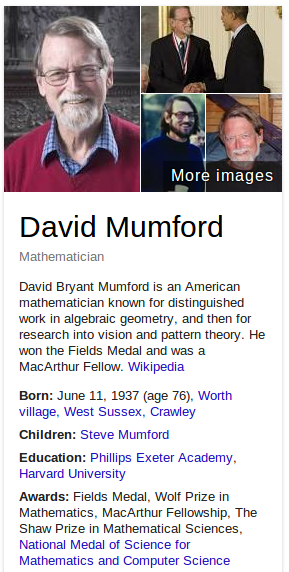
\includegraphics[width=\textwidth]{mumford}
\column{.7\textwidth}
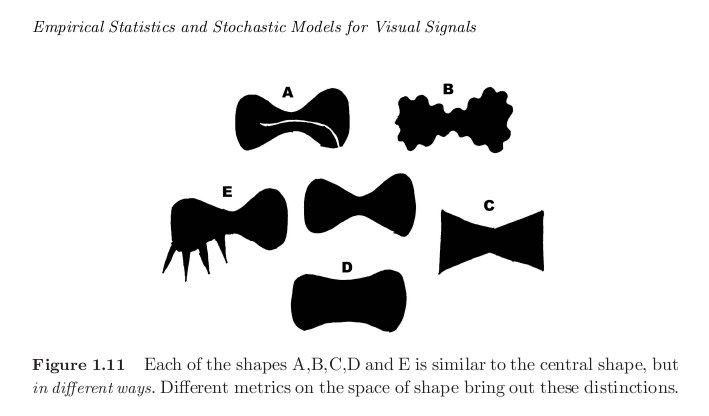
\includegraphics[width=\textwidth]{mumford_fig}
\end{columns}
\end{frame}

%\begin{frame}
%\frametitle{Weighting the data}
%\begin{Huge}
%\begin{align*}
%{\bf K} = {\bf X}{\bf W}{\bf X}^T
%\end{align*}
%\end{Huge}
%\end{frame}

\begin{frame}
\frametitle{Kernel Matrices}
Linear kernel matrices may computed from the raw features.
\begin{Large}
\begin{eqnarray*}
{\bf K} = {\bf X}{\bf X}^T
\end{eqnarray*}
\end{Large}
A simple spatial feature selection may be considered as the following, where ${\bf W}$ is a diagonal matrix of ones and zeros:
\begin{Large}
\begin{eqnarray*}
{\bf K} = {\bf X}{\bf W}{\bf X}^T
\end{eqnarray*}
\end{Large}
However, ${\bf W}$ may be more complicated, for example encoding spatial smoothing, high-pass filtering or any number of other things.
\end{frame}

\begin{frame}
\frametitle{Prior knowledge about brain regions involved}
\begin{itemize}
\item The best way would be to augment the training data with data from previous studies.
\item Lack of data-sharing means this is generally not possible,\\
      so we need to extract information from publications.
\item The neuroimaging literature is mostly blobs.
\item These give pointers about how best to weight the data\\
      (${\bf W} = diag({\bf w}), w_i \in \mathbb{R}^+$).
\end{itemize}
\end{frame}

\begin{frame}
\frametitle{Weighting suspected regions more heavily}
\begin{center}
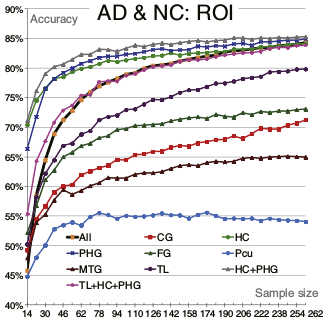
\includegraphics[width=.45\textwidth]{prior_knowledge_AD_NC}
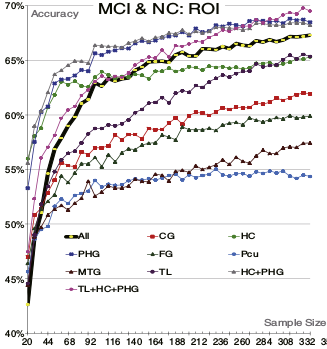
\includegraphics[width=.45\textwidth]{prior_knowledge_MCI_NC}\par
\begin{tiny}
Chu et al. ``Does feature selection improve classification accuracy? Impact of sample size and feature selection on classification using anatomical magnetic resonance images''.  NeuroImage 60:59--70 (2012).\par
\end{tiny}
\end{center}
\end{frame}


\begin{frame}
\frametitle{Smoothing can help}
\begin{columns}[c]
\column{0.33\textwidth}
If we know that higher frequency signal is more likely to be noise.\par
\begin{Large}
\begin{eqnarray*}
{\bf K} = {\bf X}{\bf W}{\bf X}^T
\end{eqnarray*}
\end{Large}

${\bf W}$ no longer diagional.
\column{0.67\textwidth}
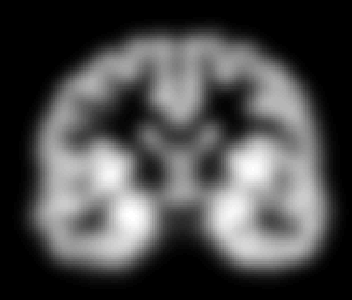
\includegraphics[width=\textwidth]{brain-GM-smo}
\end{columns}
\end{frame}


%\begin{frame}
%\frametitle{Inner Products}
%This gives us an alternative way of measuring distances between vectors in a linear way, where ${\bf W}$ is symmetric and positive definite.
%\begin{eqnarray*}
%d({\bf x}_1,{\bf x}_2) = \sqrt{({\bf x}_1 - {\bf x}_2)^T {\bf W} ({\bf x}_1 - {\bf x}_2)}
%\end{eqnarray*}
%
%The operation ${\bf W}{\bf x}^T$ may be performed as a convolution.  For example, when dealing with 2D data, we may wish to convolve with a Laplacian operator.
%\begin{eqnarray*}
%{\nabla}^2 {\bf x} = {\bf x} \ast \begin{pmatrix} 0 & -1 & 0\cr -1 & 4 & -1\cr 0 & -1 & 0\end{pmatrix}
%\end{eqnarray*}
%
%Similarly, spatial smoothing may also be envisaged within the same framework.
%%Note that the actual form of ${\bf W}$ can vary, so we need to figure out what metric tensor is optimal.
%\end{frame}

